\documentclass[10pt,oneside]{article}
\usepackage{polski}
\usepackage{fancyhdr} %numerowanie i toppery
\usepackage{lastpage} %ostatnia strona
\usepackage{indentfirst} %wcięcie
\usepackage{tikz}
\usepackage{graphicx}
\usepackage[section]{placeins}

\title{Specyfikacja implementacyjna - RealityForetell}
\author{Adrian Bączek, Łukasz Leszczyński}
\date{14.11.2019}

\pagestyle{fancy}
\fancyhf{}


\begin{document}
	\maketitle
	
	\rfoot{
		\begin{flushright}
			v1.0
		\end{flushright}
	}
	
	\thispagestyle{fancy}
	
	\newpage
	
	\rfoot{
		\begin{center}
			Strona \thepage \hspace{1pt} z \pageref{LastPage}
		\end{center}
	}
	
	\tableofcontents
	
	\newpage
	
	\section{Wstęp}
	\subsection{Cel dokumentu}
	Celem bezpośrednim dokumentu jest ułatwienie samodzielnego odtworzenia programu, wyznaczającego optymalną strukturę zakładu penitencjarnego, przez programistów we własnym środowisku. Celem pośrednim stworzonego dokumentu jest rozszerzenie wiedzy użytkownika o tematykę algorytmów ewolucyjnych.
	\subsection{Odbiorca dokumentu}
	Dokument stworzony został z myślą o ludziach szukających własnej ścieżki samorozwoju, pragnących pogłębić wiedzę na temat programowania, istoty algorytmów genetycznych oraz ich szerokiego wachlarza zastosowań. 
	
	\section{Środowisko deweloperskie}
	Sekcja zawiera podstawowe informacje na temat środowiska, w którym powstawało oprogramowanie, ułatwiające wierne jego lokalne odtworzenie przez odbiorcę.
	\begin{center}
		Parametry komputera i środowiska programistycznego:
		\newline \newline
		\begin{tabular}{|c|c|} \hline
			Procesor & Intel(R) Core(TM) i5-3230M CPU@2.60 GHz
			\\[10pt] Pamięć RAM & 8GB DDR3 1600 MHz
			\\[10pt] System operacyjny & Windows 10 Home v10.0.18362
			\\[10pt] Język programowania & Java
			\\[10pt] Środowisko programistyczne & IntelliJ IDEA Community Edition 2019.2.1 x64
			\\[10pt] Wersja pakietu Java Development Kit & 1.8.0\_211
			\\[10pt] Wersja maszyny wirtualnej języka Java & 25.211-b12\\ \hline
		\end{tabular}
	\end{center}
	
	\section{Zasady wersjonowania}
	Wersjonowanie projektu w opisywanym dokumencie odbywać się będzie w~następujący sposób. Zaplanowanych zostało 10 wydań oprogramowania, kończąc prace nad kodem na wersji 1.0. Według założeń projektu, aktualna wersja oprogramowania dostępna będzie w gałęzi głównej repozytorium (,,master"), zaś każdy ,,release" przygotowywany będzie na osobnej gałęzi oznaczonej odpowiednią dla siebie etykietą. Po zamknięciu prac konkretnego etapu rozwoju oprogramowania nastąpi połączenie odpowiedniej gałęzi z gałęzią główną ,,master". Zastosowanie takiej strategii prowadzenia prac umożliwi jednoczesny dostęp do stabilnej wersji oprogramowania jak i jego rozszerzania o nowe funkcjonalności.
	
	\subsection{Wydania oprogramowania}
	W ramach projektu przewidziane następujące wydania (ang. Release):
	\begin{description}
		\item[0.1.0] \hfill \\Stworzenie pakietów z zainicjowanymi klasami.
		\item[0.2.0] \hfill \\Stworzenie ekranów wchodzących w interakcję z użytkownikiem.
		\item[0.3.0] \hfill \\Implementacja kontrolerów dla ekranów z pakietu ,,GUI.Templates".
		\item[0.4.0] \hfill \\Implementacja modelów klas z pakietu ,,models".
		\item[0.5.0] \hfill \\Implementacja interfejsu ,,GeneticAlgorithm" oraz metod ,,rateIndividual" i ,,createNextGeneration" w ,,SchemeGenerator".
		\item[0.6.0] \hfill \\Implementacja metod ,,filterTopIndividuals" i ,,getBestIndividualInPopulation" w module ,,SchemeGenerator".
		\item[0.7.0] \hfill \\Implementacja metody ,,getEvolvedIterations" w module ,,SchemeGenerator" oraz modułu ,,ToPngConverter" konwertującego najlepszych osobników z danego pokolenia do formatu *.png.
		\item[0.8.0] \hfill \\Implementacja modułu zapisującego przekonwertowane osobniki do katalogu ,,Schemes".
		\item[0.9.0] \hfill \\Przygotowanie testów jednostkowych.
		\item[1.0.0] \hfill \\Finalna wersja programu, stworzenie pliku wykonywalnego ,,RealityForetell.jar".
	\end{description}
	
	\FloatBarrier
	\section{Struktura programu i diagram klas}
	Rozdział opisuje dokładną strukturę modułów wchodzących w skład oprogramowania.
	
	\subsection{Pakiet ,,Management"}
	\begin{itemize}
		\item Master - klasa główna, posiadająca metodę inicjalizującą działanie programu ,,main()"
		\item GeneticAlgorithm - interfejs posiadający nagłówki metod koniecznych do poprawnego działania programu
		\item SchemeGenerator - moduł odpowiadający za mechanizm generowania planu zakładu bazujący na algorytmie ewolucyjnym. Odpowiadać będzie on za selekcję najlepszego osobnika z konkretnej generacji oraz za stworzenie populacji następnego pokolenia do rozważenia.
		\item Conditions - moduł odpowiadający za zebranie, a następnie przechowanie, podanych na wejściu, warunków jakie musi spełnić zaprojektowany zakład.
	\end{itemize}
	
	\subsection{Pakiet ,,Models"}
	\begin{itemize}
		\item Camera - moduł reprezentujący kamerę.
		\item Window - moduł reprezentujący okno.
		\item LightBulb - moduł reprezentujący pojedynczą lampkę oświetlającą zakład.
		\item PrisonWard - moduł będący szkicem planu pryczy więziennej.
		\item MonitoringRoom - moduł będący odpowiednikiem kącika monitorującego.
		\item SanitarNook - moduł będący szkicem kącika sanitarnego.
		\item Door - moduł reprezentujący drzwi.
		\item PrisonScheme - moduł będący szkicem zakładu penitencjarnego (jednocześnie szkicem osobnika wykorzystywanego w algorytmie genetycznym).
	\end{itemize}
	
	\subsection{Pakiet ,,GUI.Controllers"}
	\begin{itemize}
		\item StartMenu - kontroler odpowiedzialny za logikę ekranu startowego. Zawiera dwie metody - onStartButtonClick() oraz onQuitButtonClick() - odpowiedzialne za odpowiednio przekierowanie do ekranu przyjmującego parametry od użytkownika oraz zamknięcie aplikacji na jego życzenie.
		\item DataForm - kontroler odpowiedzialny za logikę ekranu pobierającego dane od użytkownika. Zawiera on metody walidujące otrzymane parametry (wymiary zakładu penitencjarnego, ilość prycz więziennych, zasięg kamer). W~przypadku braku podania konkretnego parametru użytkownik jest proszony o jego podanie (analogicznie dla błędnej wartości, o jego poprawienie).
		\item Visualization - kontroler odpowiedzialny za prezentowanie wygenerowanych wyników na ekranie. Zawiera metody zmieniające aktualnie prezentowany rezultat na poprzedni/następny oraz metodę kończącą działanie programu.
	\end{itemize}
	\begin{figure}[!ht]
		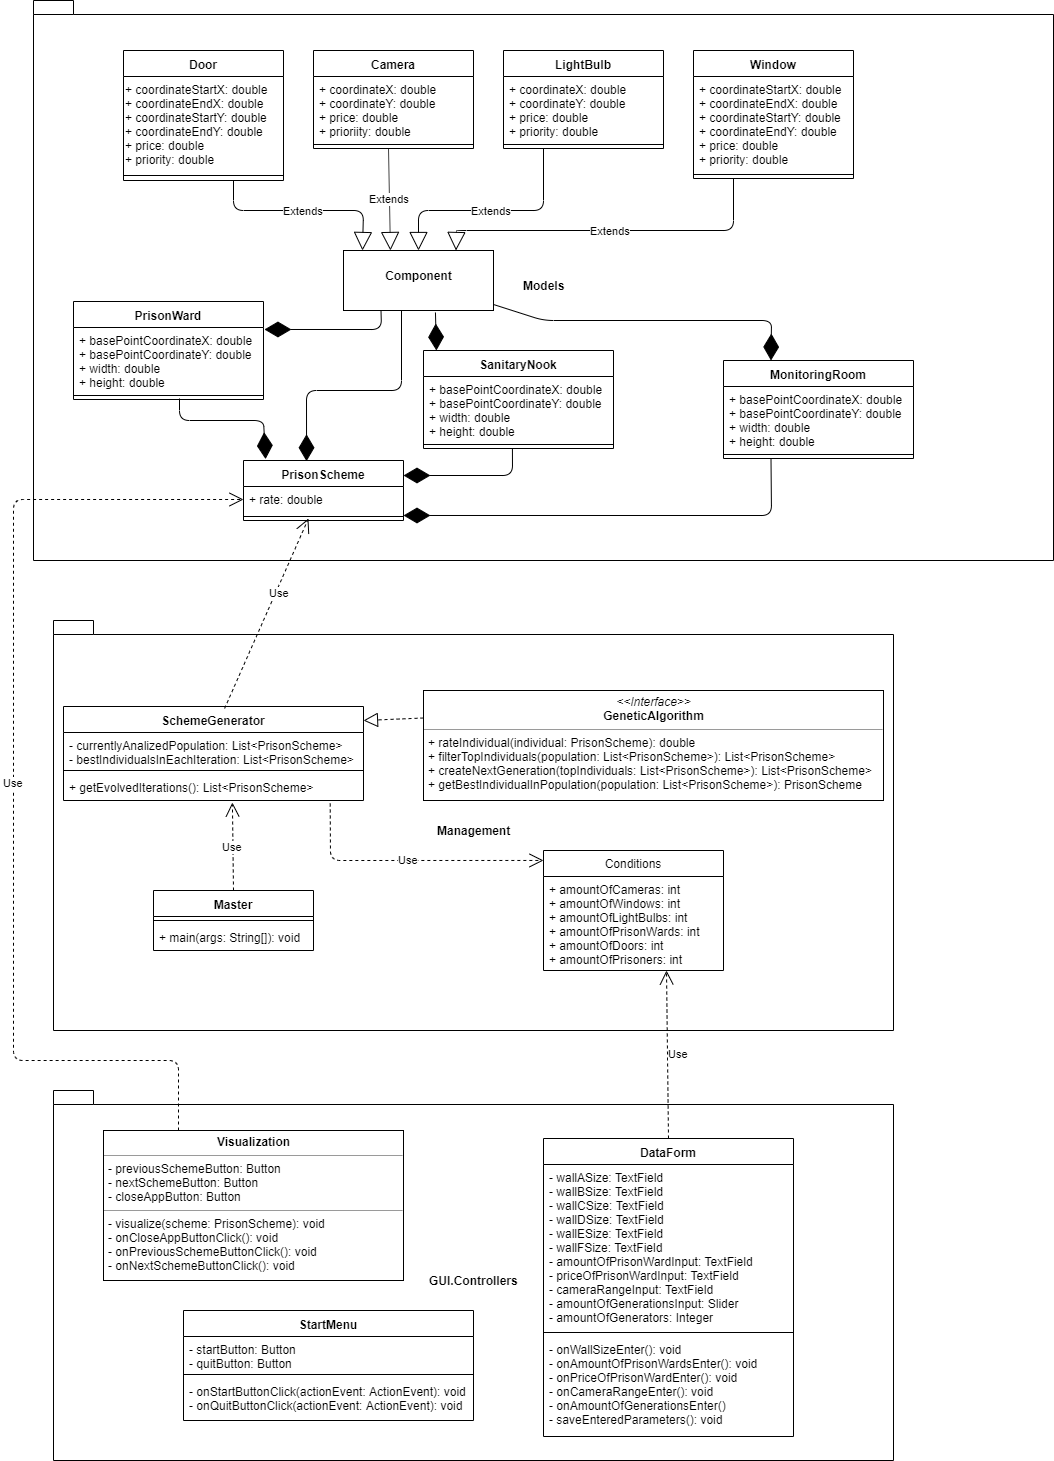
\includegraphics[width=0.9\columnwidth]{Class_diagram_Reality_Foretell.png}
		\caption{Diagram klas stosowanych w programie ,,RealityForetell".}
	\end{figure}
	
	\section{Rozwiązanie zadania}
	
\end{document}